
%(BEGIN_QUESTION)
% Copyright 2006, Tony R. Kuphaldt, released under the Creative Commons Attribution License (v 1.0)
% This means you may do almost anything with this work of mine, so long as you give me proper credit

Temaet {\it iboende karakteristikk} versus {\it installert karakteristikk} for prosessreguleringsventiler har en interessant parallell i halvlederelektronikk: transistorers oppførsel under ideelle (konstant forsyningsspenning) versus realistiske (belastede) forhold:

$$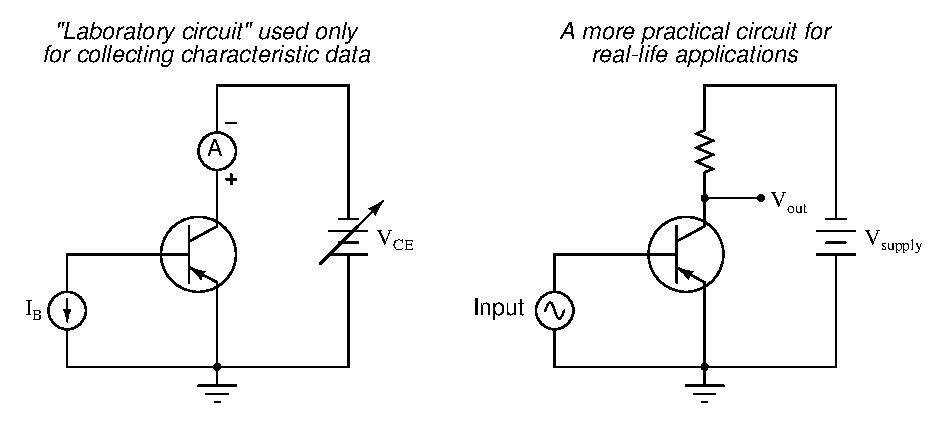
\includegraphics[width=15.5cm]{i01387x01.eps}$$

For å forstå hvordan ideell transistoroppførsel overføres til den virkelige (``installerte'') verdenen i en forsterkerkrets, kan vi tegne noe som kalles en {\it lastlinje} i samme graf som transistorens karakteristikkurver.

Forklar hva en ``lastlinje'' er, og hva den betyr for en transistorkrets.

\underbar{file i01387}
%(END_QUESTION)





%(BEGIN_ANSWER)

En ``lastlinje'' beskriver hvor mye spenning som er tilgjengelig for å drive en transistor ved en gitt kollektorstrøm:

$$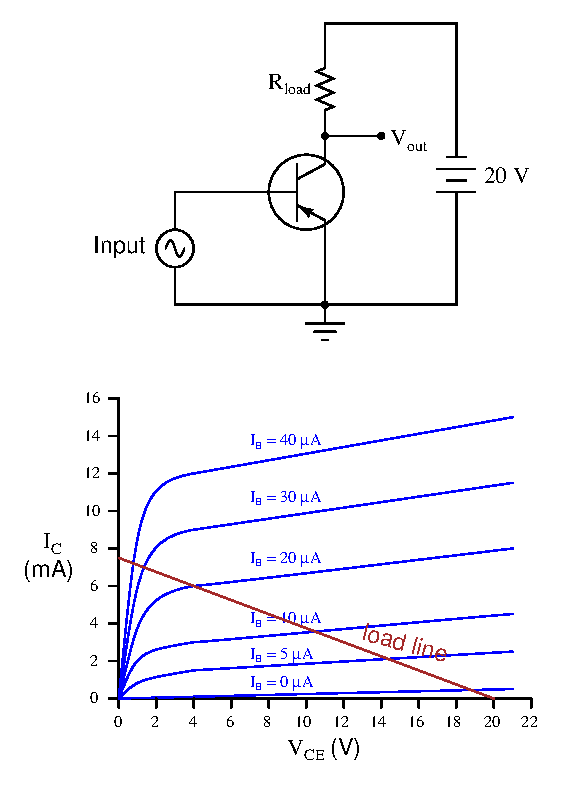
\includegraphics[width=15.5cm]{i01387x02.eps}$$

\vskip 10pt

Merk: Lastmotstanden som antydes av lastlinjen i grafen over er 2.67 k$\Omega$.

%(END_ANSWER)





%(BEGIN_NOTES)


%INDEX% Electronics review: load lines
%INDEX% Final Control Elements, valve: characterization

%(END_NOTES)

